\chapter{Алгоритм дифференциальной эволюции для задачи оптимизации фазированных антенных решеток}\label{sec:radio}

\section{Базовая реализация}\label{sec:de:default}

Эволюционные алгоритмы~(ЭА) — один из наиболее широко используемых методов решения сложных задач оптимизации. Несколько вариантов этих стратегий были разработаны и применены во многих областях, таких как наука, экономика и инженерия. Среди них дифференциальная эволюция~(ДЭ)~\cite{storn:de} — одна из наиболее эффективных стратегий непрерывной оптимизации. Более того, ДЭ была признана стратегией-победителем нескольких конкурсов по оптимизации~\cite{das:de}. Подобно другим эволюционным алгоритмам, ДЭ вдохновлен естественным процессом эволюции и включает в себя применение мутаций, рекомбинаций и селекции. Основная особенность метода ДЭ заключается в том, что он учитывает различия среди векторов, присутствующих в популяции, для изучения пространства поиска. В этом смысле он похож на оптимизаторы Nelder-Mead~\cite{nelder:simplex} и Controlled Random Search~(CRS)~\cite{price:global}.

ДЭ -- стохастический алгоритм на основе популяции, поэтому он итеративно выводит несколько наборов решений-кандидатов. В ДЭ такие решения-кандидаты обычно называются векторами. В базовом варианте ДЭ для каждого члена популяции~(их называют целевыми векторами) создается новый мутантный вектор. Затем мутантный вектор комбинируют с целевым вектором для создания пробного вектора. Наконец, применяется фаза селекции для выбора выживших. Таким образом, несколько поколений популяции эволюционируют, пока не будет достигнут критерий остановки. В поколении $G$ $i$-й вектор популяции обозначается как $\textbf{X}_{i,G} = [x_{1,i,G}, x_{2,i,G}, ..., x_{D,i,G}]$. Ниже приведены более подробные сведения о каждой фазе ДЭ.

Эксперименты показывают~\cite{storn:de_practical}, что в целом эволюция популяции соответствует динамике случайного облака точек, движущегося как целое вдоль рельефа оптимизируемой функции, повторяя его характерные особенности. В случае попадания в овраг <<облако>> принимает форму этого оврага и распределение точек становится таким, что математическое ожидание разности двух случайных векторов оказывается направленным вдоль длинной стороны оврага. Это обеспечивает быстрое движение вдоль узких вытянутых оврагов, тогда как для градиентных методов в аналогичных условиях характерна колебательная динамика «от стенки к стенке». Приведенные эвристические соображения иллюстрируют наиболее важную и привлекательную особенность алгоритма ДЭ -- способность динамически моделировать особенности рельефа оптимизируемой функции. Именно этим объясняется замечательная способность алгоритма быстро проходить сложные овраги, обеспечивая эффективность даже в случае сложного рельефа.

\paragraph*{Инициализация.}

ДЭ обычно начинает процесс оптимизации со случайно инициированной популяции, состоящей из $D$ векторов. Поскольку информация о перспективности различных регионов обычно отсутствует, применяются однородные генераторы случайных чисел: $j$-я компонента $i$-го вектора инициализируется как $x_{j, i, 0} = a_{j} + rand_{i,j}[0, 1](b_j - a_j )$, где $rand_{i,j} [0, 1]$ -- равномерно распределенное случайное число, лежащее между 0 и 1.

\paragraph*{Мутация.}

Для каждого целевого вектора создается мутантный вектор. В настоящее время известно несколько способов выполнения этого процесса. В классическом варианте ДЭ применяется стратегия $rand/1$. В этом случае мутантный вектор $\textbf{V}_{i,G}$ создается следующим образом:

\begin{equation}\label{eq:de_mut}
  \textbf{V}_{i,G} = \textbf{X}_{r1,G} + F \times (\textbf{X}_{r2,G} - \textbf{X}_{r3,G}), r_1 \neq r_2 \neq r_3
\end{equation}

Индексы $r_1, r_2, r_3 \in [1, D]$ -- различные целые числа, случайно выбранные из диапазона [1, D]. Кроме того, все они отличаются от индекса~$i$. Важно учитывать, что разница между векторами масштабируется числом F, которое называется силой мутации и обычно определяется в интервале [0.4, 1].

\paragraph*{Рекомбинация.}

Для объединения информации о различных решениях-кандидатах и с целью увеличения разнообразия применяется оператор кроссинговера. В частности, каждый целевой вектор~$\textbf{X}_{i,G}$ смешивается с соответствующим ему мутантным вектором~$\textbf{V}_{i,G}$ для создания пробного вектора $\textbf{U}_{i,G} = [u_{1,i,G}, u_{2,i,G}, ..., u_{D,i,G}]$. Наиболее типичным кроссовером является биномиальный, который работает следующим образом:
\begin{equation}\label{eq:de_crossover}
  \textbf{U}_{j,i,G} =
    \begin{cases}
     v_{j,i,G}, & \mbox{если~} rand_{i,j}[0, 1] \leq CR \mbox{~или~} j = j_{rand} \\
     x_{j,i,G}, & \mbox{иначе}
    \end{cases},
\end{equation}
где $rand_{i,j}[0, 1]$ -- равномерно распределенное случайное число, $j_{rand}$ -- случайно выбранный индекс, который гарантирует, что $\textbf{U}_{i,G}$ наследует хотя бы одну компоненту от $\textbf{V}_{i,G}$, $CR \in [0, 1]$ -- интенсивность кроссовера.

\paragraph*{Селекция.}

Наконец, выполняется жадный отбор для определения оставшихся в живых следующего поколения. Каждый пробный вектор сравнивается с соответствующим ему целевым вектором, и выживает лучший из них:

\begin{equation}\label{eq:de_sel}
  \textbf{X}_{i,G+1} =
  \begin{cases}
    \textbf{U}_{i,G}, & \mbox{если} \tilde{F}(\textbf{U}_{i,G}) \leq \tilde{F}(\textbf{X}_{i,G}) \\
    \textbf{X}_{i,G}, & \mbox{иначе}.
  \end{cases}
\end{equation}

Следовательно, каждый член популяции либо становится лучше по целевой функции, либо остается с тем же значением целевой функции в следующем поколении.

\section{Гибридный вариант алгоритма}
Будучи примененной к различным примерам из~\cite{tyu:daor}, описанный выше базовый вариант алгоритма  дифференциальной эволюции зачастую не мог обнаружить даже допустимых решений за все отведенное ему время. Чтобы избежать этой тенденции, в данной работе предложен гибридный вариант ДЭ с использованием градиентного метода, масштабированием решений в допустимую область и адаптацией штрафа, учитывающий специфику решаемой задачи.

Гибридная модификация может быть описана следующей общей схемой:

\begin{flushleft}
\small
$i$ := \verb"номер текущей итерации" \\
$i_0$ := \verb"номер итерации, на которой было получено улучшение рекорда"\\
$D$ := \verb"размер популяции"\\
$Grad$ := \verb"градиентный алгоритм"\\
$X$ := \verb"лучшая особь популяции"\\

\textit{если} $i > D$ \textit{И} $i > 2 * i_0$ \textit{то} \{\\
\leftskip=12pt
    $X_{next} := Grad(X)$\\
    \textit{если} $X_{next}$ = $X$ \textit{то} \verb"завершить выполнение", $X$ \verb"является решением"\\
    \textit{иначе} \{\\
    \leftskip=24pt
        $X = X_{next}$\\
        $i_0 = i$\\
        \leftskip=12pt
    \}\\
    \leftskip=0pt
\}
\end{flushleft}
Условие $i > 2 * i_0$ определяет, происходило ли улучшение популяции за определенное количество итераций. Условие $i > D$ гарантирует, что на начальных итерациях ДЭ не будет принято решение о запуске градиентного алгоритма~\cite{eremeev:restart}.

% TODO: переформулировать
%Для рассматриваемой задачи существует преобразование, позволяющее привести к допустимой области решение $\textbf{x}$, которое нарушает только ограничивающие неравенства задачи~(\ref{eq:task3}) вида $\textbf{x}^{T}\textbf{H}^{(k)}\textbf{x} \leq 1$:

%\begin{equation}
%    \textbf{x}': =\alpha(\textbf{x})^{-1/2} \textbf{x} ,
%    \label{eq:scale}
%\end{equation}
%где $\alpha(\textbf{x}):=\max_{k=\overline{1,n}} \textbf{x}^T \textbf{H}^{(k)}\textbf{x}$. Поскольку как целевая функция, так и ограничения представлены квадратичными формами, применение такой операции приведет к пропорциональному уменьшению в~$\alpha(\textbf{x})$ раз значений каждой из квадратичных форм. Другими словами, если в некоторой точке $\textbf{x}$ значения каждой из квадратичных форм, задающих ограничения, больше 0, причем значения некоторых из них больше 1, то по формуле (\ref{eq:scale}) можно определить множитель, умножение которого на вектор $\textbf{x}$ ведет к тому, что наибольшее из значений квадратичных форм, задающих ограничения, будет равно 1. 
Описанная в разделе~\ref{sec:scaling} процедура масштабирования в допустимую область применяется для выбора начального решения, а также для масштабирования каждого нового решения перед оценкой его качества в алгоритме ДЭ. При этом если решение до масштабирования имело большие нарушения ограничений, то после масштабирования его целевая функция существенно изменяется, как правило в сторону снижения качества. На этом принципе основано адаптивное правило подбора штрафного коэффициента, описываемое далее.

Кроме того, для улучшения качества решений в гибридном варианте предлагается динамическое увеличение штрафного коэффициента:

\begin{flushleft}
\small

$i$ := \verb"номер текущей итерации" \\
$i_0$ := \verb"номер итерации, на которой было получено улучшение рекорда"\\
$i_1$ := \verb"номер итерации, на которой произошло предыдущее увеличение штрафа"\\
$D$ := \verb"размер популяции"\\
$r$ := \verb"штрафной коэффициент"\\

\textit{если} $i > D$ \textit{И} $i > 1.5 * i_0$ \textit{И} $i > 2 * i_1$  \textit{то} \{\\
\leftskip=12pt
    $r := 2r$\\
    $i_1 := i$\\
    \leftskip=0pt
\}
\end{flushleft}

Здесь условие $i > D$ гарантирует, что на начальных итерациях не будет принято решение об увеличении штрафа, а условие $i > 1.5 * i_0$ - что лучшее значение популяции не было улучшено за определенное количество итераций. Условие $i > 2 * i_1$ <<замедляет>> следующее срабатывание критерия.
Таким образом, при отсутствии существенных улучшений качества решений происходит увеличение штрафного коэффициента. С учетом масштабирования особей в допустимую область, это приводит к выживанию особей с меньшим нарушением ограничений и позволяет улучшить качество получаемых решений.

\section{Вычислительный эксперимент}\label{sec:exp:de}

Вычислительный эксперимент был поставлен для задач, рассмотренных в~\cite{tyu:daor,tyunin:oniip}. В данной статье ШВИК, ШВДК, СВДК обозначают решетки кольцевой структуры. Далее следует указание количества элементов (8 или 16). Через тире -- расстояние от центра излучателя до центра решетки (15, 20, 25, 30, 37). Для ШВД приводится плотность противовесов (например, 3:3). Поскольку современные ЭВМ на аппаратном уровне поддерживают вычисление в параллельном режиме, рассматриваемый здесь алгоритм ДЭ был адаптирован под эту особенность: за один запуск алгоритма производится 4 параллельных выполнения, а на выход подается лучшее решение. Это позволяет использовать возможности современных ЭВМ для получения более качественных решений. В таблице~\ref{tab:results_de} результаты, полученные с помощью ДЭ, сравниваются с результатами коммерческого решателя BARON и в пакете GAMS.
%В колонке BARON* показаны результаты, полученные решателем BARON при учете фазовой симметрии. Для ДЭ также были произведены эксперименты при учете симметрии, однако, их результаты практически идентичны результатам ДЭ без учета симметрии, поэтому, в таблице~\ref{tab:results_de} они не приводятся. Поскольку решатель BARON в пакете GAMS в режиме по умолчанию имеет ограничение по времени 1000с., ДЭ также использует этот лимит.
Решатель BARON, также как ДЭ, имеют ограничение по времени счета 1000с (эта длительность выбрана из практических соображений, т.к. она сопоставима с временем построения исходных данных с использованием системы NEC, и совпадает с ограничением по времени, выбранным в~\cite{tyu:daor}).
%В случае, если ДЭ получит решение раньше установленного временн\'{о}го ограничения, производится повторный запуск алгоритма до тех пор, пока это ограничение не будет исчерпано. За
В случае нескольких запусков ДЭ за отведенное время, за решение принимается лучшее из найденных за 1000с. Для оценки среднего значения целевой функции на выходе ДЭ производилась серия из 10 независимых испытаний по 1000с в каждом. Результаты эксперимента при выборе типичных значений настраеваемых параметров ДЭ (популяция из 100 особей, $F=0.6$, $CR=0.6$) представлены в  таблице~\ref{tab:results_de}. Значения целевой функции в таблице округлены до целых. Полужирным шрифтом выделены случаи, когда указанное значение целевой функции не менее, чем на 1\% выше, чем у другого алгоритма. Вычисления производидись на ЭВМ с процессором Intel i7 (тактовая частота:
2.8ГГц), ОЗУ: 16Гб.

\begin{table}[!h]

\centering
\caption{ Результаты экспериментов, полученные с помощью ДЭ и BARON}
\begin{tabular}{|c|c|c c|c c|}
    \hline
    \multirow{2}{*}{\textbf{Тип}} & \textbf{ДЭ} & \multicolumn{2}{|c|}{\textbf{BARON}} \\
    & \textbf{$\tilde{F}$} & \textbf{$\tilde{F}$} & \textbf{t, c}  \\
    \hline
    ШВИ 2х2         & ${139}$   & 139    & 0.12      \\
    ШВИ 3х3         & ${580}$   & 580    & 0.34       \\
    ШВД 2х2         & ${463}$   & 463    & 0.27     \\
    ШВД 3х3         & ${924}$   & 925    & 0.34        \\
    СВД 2х2         & ${361}$   & 361    & 0.16         \\
    СВД 3х3        & 1163  & $\mathbf{1261}$   & 0.38     \\
    СВД 5х5         & $\mathbf{7132}$  & 6716   & 1000   \\
    СВД' 2х2       & 198   & $\mathbf{253}$    & 0.25         \\
    СВД' 3х3       & 834   & $\mathbf{1153}$   & 1.4          \\
    СВД' 5х5        & $\mathbf{2755}$  & 33     & 217.94     \\
    ШВИК 8-15(3:3)  & ${218}$   & 218    & 0.23       \\
    ШВИК 16-15(3:7) & ${732}$   & 734    & 1.37     \\
    ШВИК 8-15(2:3)  & $\mathbf{1664}$     & -   & 14.62     \\
    ШВДК 8-20       & ${1454}$  & 1454   & 2.78       \\
    ШВДК 8-30       & ${2421}$  & 2421   & 1.47     \\
    СВДК 8-25       & ${732}$   & 734    & 0.23        \\
    СВДК 8-37       & ${1486}$  & 1486   & 0.23      \\
    \hline
\end{tabular}
\label{tab:results_de}
\end{table}

%Также в результате проведенных экспериментов были получены другие результаты, не отраженные в таблице~\ref{tab:results_de} для краткости изложения.
Aналогичные испытания производились и с помощью решателя ANTIGONE в пакете GAMS, однако, было выявлено, что в режиме по умолчанию данный решатель на всех задачах выдал нулевое решение, кроме СВД~2х2, где решение по целевой функции совпадало с результатом BARON.
Также, в результате проведенных экспериментов было обнаружено, что динамическая адаптация штрафного коэффициента позволяет ДЭ достичь более качественных решений, что особенно заметно в тех случаях, когда результаты ДЭ и BARON близки по качеству.

С целью изучения возможности ускорения работы решателей за счет учета специфики задачи были проведены дополнительные исследования
структуры рассматриваемых примеров с точки зрения линейных симметрий этих задач~\cite{yurkov:symmetry}. Ранее было отмечено (см.~\cite{tyu:daor}), что решения рассматриваемой задачи эквивалентны с точностью до сдвига фаз во всех излучателях на равную величину.
Учет данной симметрии (для краткости называемой <<фазовой симметрией>>) может быть реализован фиксацией в ноль одной из переменных задачи, например, $x_1=0$. В результате добавления такого ограничения к условиям задачи число переменных сокращается на единицу и можно предположить, что это сократит время вычислений для известных алгоритмов. Нами поставлены вопросы о том, действительно ли происходит сокращение времени вычислений и о существовании других семейств симметрий, которые могли бы еще более сократить пространство поиска решаемой задачи.

Для ответа на первый вопрос на всех тестовых примерах был найден коэффициент ускорения решателя BARON, получаемый от фиксации $x_1=0$. Результаты представлены на рисунке~1 (здесь отсутствует задача СВД' 5х5, где алгоритм с фиксацией затратил существенно большее время, но при этом нашел решение с большим на 10\% значением целевой функции, а также задача ШВИК 8-15(2:3), в которой решения не были найдены в обоих случаях).     В большинстве примеров фиксация переменной привела к ускорению работы алгоритма, среднее ускорение по представленным здесь задачам составило 0.95, что говорит о целесообразности фиксации в ноль одной из переменных при использовании решателя. Аналогичный эксперимент с алгоритмом ДЭ и решателем ANTIGONE не показал существенного улучшения качества решений или их ускорения в результате фиксации~$x_1$.

Для ответа на второй вопрос был проведен поиск непрерывой группы линейных симметрий в рассматриваемых примерах, как описано ниже в приложении. В результате было установлено, что других непрерывных семейств линейных симметрий в рассматриваемых примерах не существует. Вопрос о поиске дискретных симметрий пока остается открытым.

\begin{figure}
\center{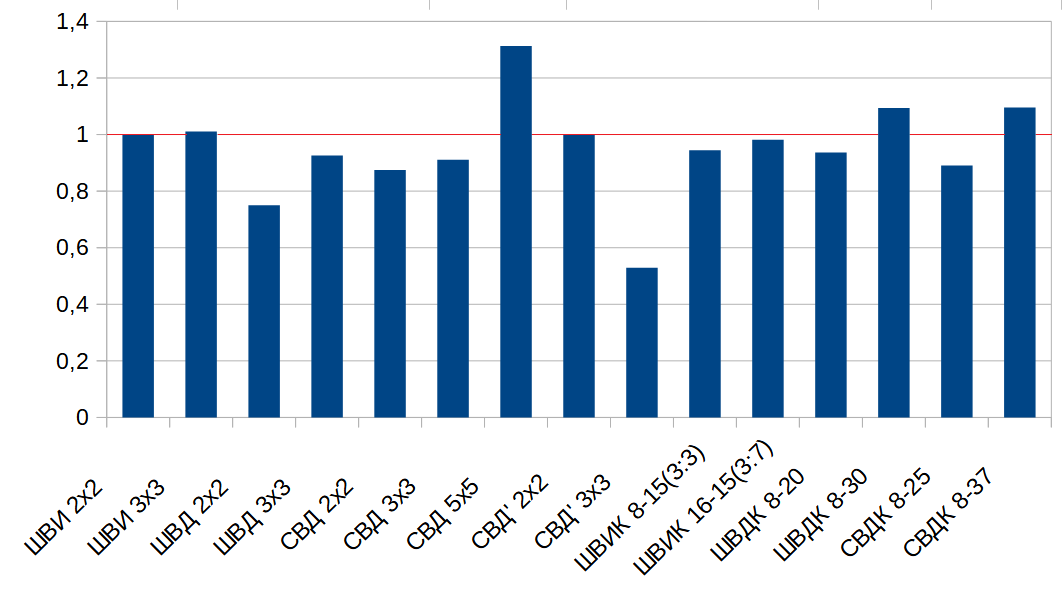
\includegraphics[width=0.6\linewidth]{ratio.png}}
\caption{Отношение длительности вычислений с фиксацией первой координаты к исходной длительности вычислений}
\label{ris:ring}
\end{figure}

Из проведенных экспериментов можно сделать следующие выводы:
\begin{itemize}
  \item Разработанный в рамках данной работы гибридный вариант ДЭ показывает конкурентоспособные результаты по сравнению с коммерческим решателем BARON в режиме его настроек по умолчанию, при этом преимущество ДЭ наблюдается на задачах с наибольшей размерностью (25 и 16 переменных).
  \item Решатель ANTIGONE в режиме его настроек по умолчанию в большинстве тестовых примеров возвращает нулевое решение.
  \item Учет фазовых симметрий задачи~(\ref{eq:task1}), как правило, позволяет ускорить работу решателя BARON.
  \item Других непрерывных семейств линейных симметрий в рассматриваемых задачах не существует.
\end{itemize}

\section{Заключение}\label{sec:conclusion}

В рамках данной работы был разработан гибридный вариант алгоритма дифференциальной эволюции с исполььзованием градиентного алгоритма и адаптацией штрафа. Показано, что разработанный вариант ДЭ демонстрирует конкурентоспособные результаты.

В целях ускорения работы алгоритмов для рассмотренных задач была применена методика анализа наличия группы непрерывных симметрий, в результате которой было обнаружено наличие только фазовой симметрии. Было произведено сравнение гибридного алгоритма и коммерческих решателей с учетом обнаруженной симметрии и без нее. Выявлено, что учет симметрии может привести к ускорению работы решателя BARON.

Результаты данного исследования опубликованы в~\cite{tyu:de_sym}.
